\section{Domain Overview}

\subsection{Introduction to Distributed Systems}

Distributed Systems are a type of system which are designed to operate in a fragmented setting. This fragmented style helps the system to distribute its workload over many computers across a network which in itself makes scaling such a system easy as adding more computers to the network. This method of scaling is called horizontal scaling. Using this kind of fragmented architecture helps to increase the reliability of the system since the likelihood of a single hardware failure knocking out the entire system gets smaller and smaller as the network grows.

In the early days, only large-scale enterprises could afford the cost of building distributed systems but in recent years with the rise of cloud computing \citep{CloudAdo16:online} creating our own distributed systems could be done with just a press of a few buttons.

\subsubsection{Microservices} \label{sec:intro-microservices}

This radical shift introduced a new paradigm of computing called Microservices. Where a bunch of small and self contain services work to-gather for a big and complex system. These services can be individually deployed and scaled. Due to this nature users can deploy replicas of a single service across many \acp{vm} and put a load balancer that will split the traffic between them. This method will allow the service to maintain availability even if multiple \acp{vm} which contain a copy of the service goes down \citep{chaczko2011availability}.

\subsubsection{Containerization}

Even though microservices helped more organizations meet a higher level of availability due to their decoupled nature. It was very difficult to manage the lots and lots of tiny services spread across hundreds of \acp{vm}. Since these services were isolated using a virtualization layer the cost and the overhead of maintaining a system like this were very high \citep{dua2014virtualization}. To mitigate this problem inspired by Logistics Industry, a new method to package an application called "Containerization" was invented. The rationale behind this technique was to package all the dependencies of the program to a single image without the operating system itself and when running share a single logically separated operating system across all the containers. So using this technique will reduce a lot of overhead in the system and also it make simple to move an application running on a local computer to a remote server due to the aforementioned dependency packaging technique.

\begin{figure}[H]
    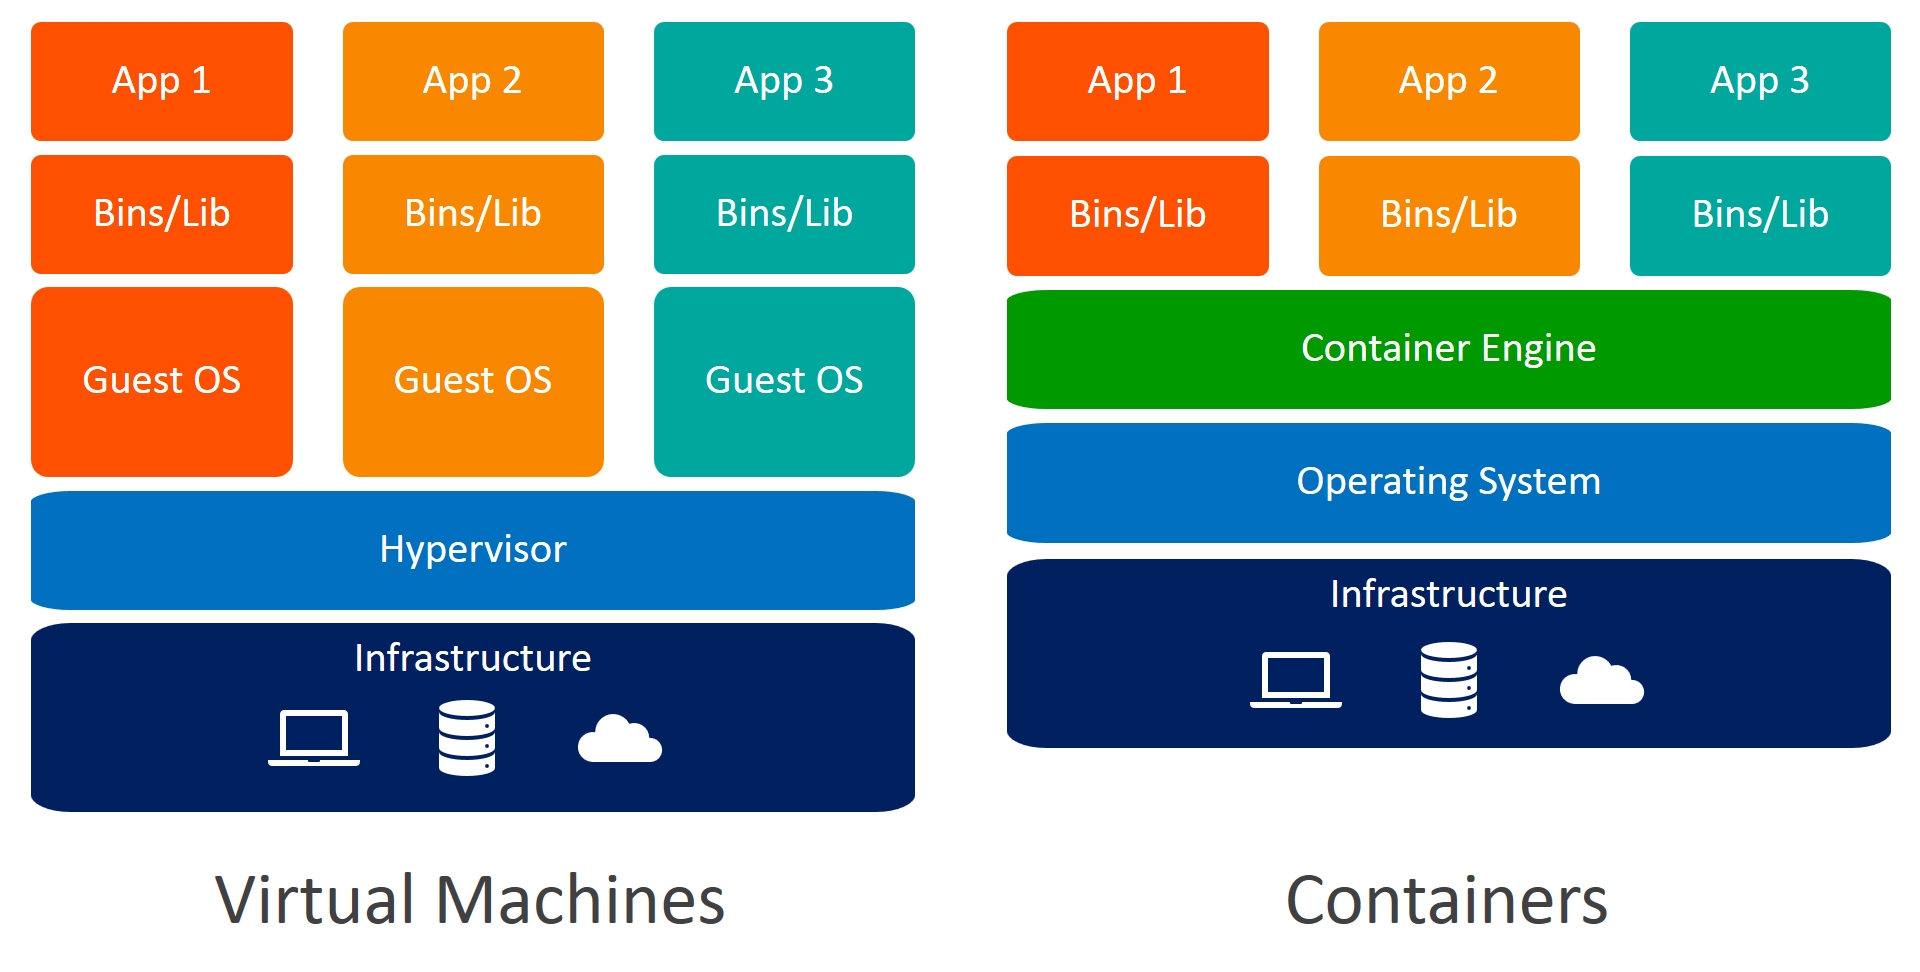
\includegraphics[width=9cm]{assets/literature-review/containers-vs-virtual-machines.jpg}
    \caption{Difference between hosting 3 apps in virtual machines vs Containers \citep{Dockervs91:online}}
\end{figure}

\subsubsection{Container Orchestration}

Even though containers solve a major headache when it comes to operating a distributed system, managing 100s of containers becomes a major challenge. The reason for this is when it comes to a large-scale distributed system, it's simply not possible to use one \ac{vm} to house all the containers. These containers need to be spread across dozes of \acp{vm} and in some cases different \ac{vm} vendors. Then networking, replication, security, and \textbf{monitoring} need to be accounted for. To solve all of these problems number of different container orchestration systems were introduced \citep{ElasticityCloudComputing}. But as per a survey done by Red Hat in July 2021, it's reviled that 88\% of people prefer to use Kubernetes as their container orchestrator while 74\% mentioned they use Kubernetes for their production workloads \citep{Kubernet59:online}.

\begin{figure}[H]
    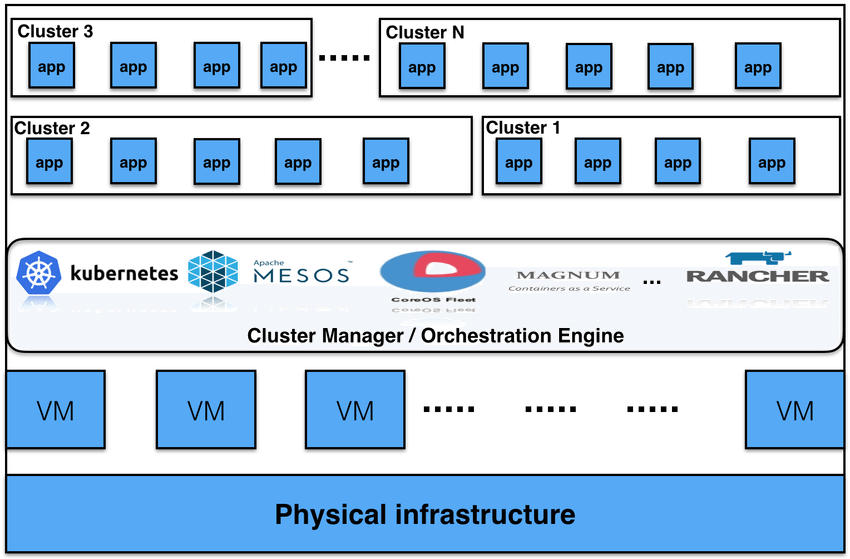
\includegraphics[width=9cm]{assets/literature-review/Container-orchestration-engines.png}
    \caption{Overview of a container orchestration engine \citep{ElasticityCloudComputing}}
\end{figure}


\subsection{Reliability Engineering}

With the rise of cloud computing, a new culture of software development called DevOps emerged. According to \cite{kim2014phoenix} philosophy behind DevOps was adopted from "Toyota Way"  \citep{liker2006toyota}. In that book author talks about "The Three Ways",
\begin{enumerate}
\item \textbf{Principles of Flow} - Workflow from left-to-right (from the requirement to production) and to maximize flow batch sizes need to be lowered.
\item \textbf{Principles of Feedback} - To increase the quality, feedback must be passed from right to left so that the entire idea to production workflow has a feedback loop. 
\item \textbf{Principles of Continuous Learning} - Every failure is a learning opportunity.
\end{enumerate}
and these three principles essentially makeups the modern DevOps culture. So a well-implemented DevOps culture on an organization will yield much better results both the quality of the system and its reliability. 

As mentioned above DevOps is considered as a culture or set of abstract principles that break down the organizational silos to achieve a higher level of agility that was considered impossible some time ago. \ac{sre}, is the implementation of this abstract concept with clearly defined roles and tasks. Their main responsibility is to keep the system running smoothly as possible and adapt the infrastructure to fit the needs of the system. To achieve this \acp{sre} rely on number automation tools, which help them from building the software to extracting real-time insights while it's running on production.


\subsection{How to Identify the Root Course of a Failure}\label{sec:how-root-course}


To identify the root course of an issue in the system, three major steps need to be passed.
\begin{enumerate}
\item Detect there is an issue with the system.
\item Find all the affected services.
\item Estimate the most probable course.
\end{enumerate}

Typically most of the distributed systems have some sort of monitoring system which collects telemetry data about the system in real-time. This allows the \acp{sre} to get a bird' eye view of the system's status. But to achieve a higher level of reliability it is crucial to keep tabs on every sub-component of the system, So it's possible to get understand its behavior at any given time. 

Even though this is the ideal scenario, this approach doesn't scale well. At some point, it's getting humanly impossible for the \ac{sre} team to keep track of all these services. So to solve this concept of \ac{sli} was introduced \citep{beyer2016site}. The idea behind this provides a quantitative measure of a very specific part of the system as it's faced to the end-users. For example request latency is one of the most commonly used \ac{sli}. This helps to lower the number of metrics \acp{sre} has to monitor but small errors that affect a minority of users could go unnoticed for months. 

To detect these kinds of issues, all the microservices in the system need to emit a lot of telemetry data and those data need to be individually processed in near real-time to catch errors early. The most widely adopted method of extra meaningful data from such data stream is setting up threshold-based alerts which will send notifications when there is a threshold violation. The main drawback to this issue is \acp{sre} has to predict both metrics that need to be monitored and "normal rates" for these metrics by looking at past data and that value has been valid for the future as well if the service is newly deployed it's really hard to get those two right. In fact on the 14th of December, 2020 all of Google's services went unresponsive due to Google's OAuth service running out of disk space and no one at Google didn't notice till user reports started flooding in \citep{Googleoutage:online}. 

Typically in distributed systems, services have a lot of interdependent connections to form the bigger system. When a dependant service is experiencing an issue for example the elevated level of request latency, it is possible for a service consuming that service to also show an elevated level of request latency. So when there is an outage or issue with the system \acp{sre} look at all the services with abnormal metric readings and try to make an educated guess of the most probable root course. This gets repeated until a real root course was found. The hardest part of this process is making the educated guesses of the most probable root courses and this requires the involvement of a system expert with a lot of experience with the target system.

\begin{figure}[H]
    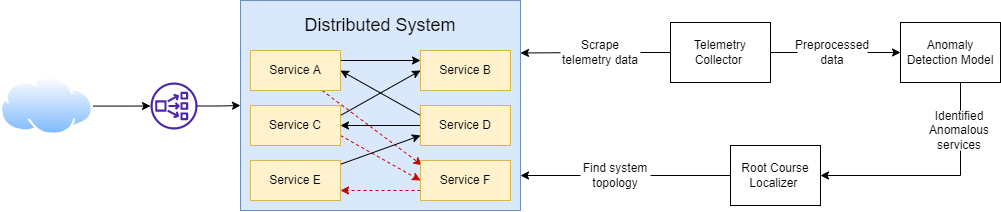
\includegraphics[width=16cm]{assets/literature-review/demo.png}
    \caption{Root course localization pipeline (self-compose)}
\end{figure}

\subsection{Artificial Intelligence for IT operations}

When it comes to IT operations like managing infrastructure and identifying the root course of failure like mentioned in the section \ref{sec:how-root-course}there tend to be a lot of both structured and unstructured data sources. \ac{aiops} is an emerging field \citep{Artifici8:online} where both data scientists and reliability engineers cooperate to build data-driven, smarter systems with help of machine learning to achieve a higher quality of service which ain't simply possible by using traditional methods due to the density and the complexity of datasets.

